\documentclass[a4paper,10pt,hidelinks]{scrreprt}
%\usepackage[utf8x]{inputenc}

% Packages =========================================
\usepackage{algorithm}
\usepackage{algpseudocode}
\usepackage{amsmath}
\usepackage{amsfonts}   		% Pakete für math. Formeln, Symbole, Ausdrücke
\usepackage{amssymb}
\usepackage[toc,page]{appendix}				% more control over appendices
\usepackage[english]{babel} 				% Anpassung für mehrsprachige Dokumente
\usepackage[usenames, dvipsnames]{color}					% Nutzung von Farben

\usepackage{float}					% notw. für explizite Setzung von Grafiken
\usepackage[T1]{fontenc} 				% Zuweisung Codierschemas für Zeichensätze
\usepackage[paper=a4paper,left=40mm,right=30mm,top=20mm,bottom=25mm]{geometry} % Randmaße
\usepackage{graphicx} 					% Einbindung externer Grafiken
\usepackage{hyperref}
%\usepackage[utf8]{inputenc}				% for german characters like "ä, ö, ü"
%\usepackage{listings}					% notwendig für Quellcode
\usepackage{lmodern}	 				% Moderne Version von Computer Modern
\usepackage{pdfpages}					% Einbindung einer pdf-Datei
\usepackage{pgfplots}
\usepackage{mdwlist}					% kompaktere Auflistungen
\usepackage{microtype}	 				% Optischer Randausgleich
\usepackage[round]{natbib}
\usepackage{doi}
\usepackage{subcaption}					% Subfigure/-tabellen
\usepackage{scrpage2}
\usepackage{tabularx}					% Textsetzung in Tabellen in p-Spalten
\usepackage{textcomp}					% Besondere Textzeichen
\usepackage{ulem}					% Unterstreichung
\usepackage{url}					% Links
\usepackage{xfrac}					% notw. für schräggestellten Bruch
\usepackage[margin=10pt,font=scriptsize,labelfont=bf,labelsep=endash]{caption}




\begin{document}
	\thispagestyle{empty}
	\begin{center}
		\Large
		\textbf{A Neuronal Model for Visually Evoked Startle Responses in Schooling Fish}\\
		
		\vspace*{1cm}
		\normalsize
		Master thesis\\
		
		\vspace{3cm}
		by\\
		Andrej Warkentin \\
		Bernstein Center for Computational Neuroscience - Berlin
		
		\vspace{2cm}
		Supervisors:\\
		Dr. Pawel Romanczuk\\
		Bernstein Center for Computational Neuroscience - Berlin\\
		Prof. Dr. Henning Sprekeler\\
		Technische Universit\"{a}t Berlin
		
	\end{center}
	\pagebreak 
	% Title Page
	\title{masterthesis}
	
	% Inhaltsverzeichnis =====================================
	\thispagestyle{empty}
	\tableofcontents		% Inhaltsverzeichnis erstellen
	\newpage
	%\cleardoublepage	% min. eine Freiseite
	
	%% Für den Hauptteil normale Seitenzahlen
	\pagestyle{useheadings}    % wieder auf normale Seitenrahmen zurück schalten
	\pagenumbering{arabic}  % Nummerierungstyp roman | arabic
	
	\begin{abstract}
		\textbf{Abstract}\\
		Many aspects of fish school behavior can be explained qualitatively by self-propelled agent models with social interaction forces that are based on either metric or topological neighborhoods.
		Recently, startling of fish has been analyzed in its dependence of the network structure \citep{Rosenthal2015} but a mechanistic model and its influence on the collective behavior is missing.
		Here we couple a model for collective behavior with a neuronal model that receives looming visual stimulus input to initiate a startle response, inspired by the neurobiologically well-studied Mauthner cell system.
		First, we analyzed the basic properties of the startle behavior of a single fish as a reaction to a looming stimulus.
		On the group level, we looked at startling frequency as well as group cohesion and polarization depending on neuronal and collective behavior parameters via simulations of the combined model.
		Our results indicate that the startling frequency strongly depends on the dynamics of the group structure, e.g. when the group approaches a boundary of the arena.
		In summary, we took first steps towards a biologically plausible model 
		for startle response initiation in the context of collective motion.
	\end{abstract}
	\newpage
	
	\chapter{Introduction}
	A common interpretation of the function of the nervous system in animals is to use the sensory 
	input in order to make appropriate actions.
	One situation where this would be useful for the animal is the sudden appearance of a predator.
	The quick response to such a sudden, unexpected stimulus is called startle response and can be 
	observed in many species \citep{Eaton1984a}.
	In fish, the startle response can take the form of freezing, where the fish	stops moving 
	entirely, or the form of an escape response, where it quickly accelerates and moves away within 
	less than a second.
	Escape responses in fish, also called fast starts, can be divided into the three stages 1) 
	first body bend, 2) second body bend and a third, variable stage where the fish either goes 
	into continuous swimming, coasting or braking \citep{Domenici2011}.
	Due to the body shape at the end of the first stage escape responses are also called C-start or 
	S-start \citep{Domenici2011}\footnote{It should be noted here that not all C-starts are escape 
	responses because the can also be involved in e.g. prey capture but we will ignore other roles 
	in the following.}.
	This thesis will focus on the C-start behavior of fish.\\
	The C-start behavior in fish has been extensively studied and one of the main reasons for this 
	is that a pair of neurons that play a major role in the initiation of the C-start, have large 
	soma and axons and are therefore relatively easy to find in experiments.
	They are called Mauthner cells (M-cells), named after Ludwig Mauthner who first found and 
	described their axons \citep{Mauthner1859}.\\
	Before going into the details of the M-cell circuit I will give a brief overview of the nervous 
	system of fish to provide some context.
	Since I will later focus on visually evoked C-starts I will go into more detail when it comes 
	to the visual pathways in the brain.
	The overall structure of the nervous system of fish is very similar to mammals.
	Starting at the caudal end there is the spinal cord with descending motor pathways and the 
	ascending sensory pathways.
	The spinal cord goes over into the hindbrain region with the medulla and the cerebellum.
	This is followed by the midbrain which comprises the rostral part of the brainstem and a roof 
	region, the tectum \cite{the chapter in encyclopedia of fish physiology}.
	The remaining forebrain consists of the diencephalon and the telencephalon.
	%TODO: say what is different in mammals/humans
	In terms of sensory organs fish are equipped with the same senses as mammals and additionally 
	have the lateral line organ that senses lower frequency signals around the body such as e.g. 
	water flow and in some cases organs that can sense electrical fields.\\
	%TODO: some transitional sentence to introduce the visual system
	Going from outside to inside, the eyes, again similar to mammals, consist of the cornea, the 
	lens surrounded by the iris and the retina followed by the photoreceptors which build the most 
	inside layer.
	In contrast to mammals the pupils of fish are not responsive to the amount of light in the 
	environment.
	Fish mostly have rods and three different cones although across species there are up to seven 
	different types of cones.
	The retina has different types of neurons that build different layers.
	The output neurons of the retina are the ganglion cells which show different kinds of tuning 
	and whose axons build the optic nerve when the exit the eye.
	%TODO: cite paper about tuning of retinal ganglion cells
	Although most fish don't have a fovea as we know it from humans there are retinal areas of 
	higher ganglion cell and photoreceptor densities \citep{Pita2015}.
	Most of the ganglion cell axons cross sides and end up in the optic tectum which is the 
	equivalent to the mammalian superior colliculus.
	While in humans much of the visual information goes further to the primary visual cortex in 
	fish the optic tectum is the main site of processing of visual information.
	Similar to cortical areas it is comprised of different layers, also receiving input from other 
	senses and other brain areas such as the telencephalon.
	The output of the optic tectum goes, among other regions, to the reticular nuclei in the 
	hindbrain where we also find the Mauthner cell and can thus come the M-cell circuit.\\
	The M-cell is located in the hindbrain and has two major dendritic branches, the ventral 
	dendrite and the lateral dendrite.
	It receives multisensory input which is divided between the two dendritic branches.
	The lateral dendrite receives auditory and lateral line input whereas the ventral dendrite 
	receives visual input via the optic tectum as described before.
	While this means that the visual input is highly processed by the networks in retina and optic 
	tectum before it arrives at the M-cell the auditory input comes directly from the auditory 
	nerve.
	This might be one of the reasons why the physiology of the auditory input has been studied in 
	more detail than the visual part.
	I will therefore continue to describe the properties of the auditory processing and will have 
	to assume that they also hold for the processing of the visual input.
	The synapses between auditory nerve and lateral dendrite are called club endings and transmit 
	auditory signals via electrical as well as chemical mechanisms which leads to Excitatory 
	Post-Synaptic Potentials (EPSPs) that consist of a fast and a slow component \citep{Korn2005}.
	At the same time the auditory nerve excites an interneuron which itself inhibits the M-cell.
	One interpretation of this feed-forward inhibition (FFI) is to increase the threshold for 
	initiating the startle response.
	But this is not the only function of these interneurons because they also inhibit the 
	contralateral M-cell as well as their contralateral counterparts \citep{Koyama2016}.\\
	This microcircuit is probably responsible for the decision of which direction to escape to.
	To illustrate why this connectivity makes sense in this decision-making context, let us 
	consider an auditory stimulus coming from the left side:
	It will inhibit the M-cell on the right side, inhibit the interneurons on the right side and 
	excite the M-cell on the left side.
	Effectively, we have an increased inhibition of the right M-cell, decreased inhibition of the 
	left M-cell and increased excitation of the left M-cell.
	Because the axons of the M-cells cross sides, an action potential of the M-cell on the left 
	side will lead to a contraction of muscles on the right side, resulting in movements of head 
	and tail away from the stimulus on the left side.\\
	There are further properties that seem to make the M-cell specialized for initiating the 
	C-start.
	Additional to the feed-forward inhibition the big size of the some of the M-cell leads to a 
	high input resistance which again increases the threshold for incoming currents to initiate an 
	action potential.
	The axon of the M-cell is unusually big as well which results in a fast signal transmission 
	when an action potential is initiated.
	The axon is also connected to interneurons that provide feedback inhibition to both M-cells.
	This is thought to prevent repetitive firing of the M-cell that fired in the first place and 
	also to prevent the contralateral M-cell to fire shortly after.
	%TODO: check if axons are connected directly to interneurons
	%TODO: check what cranial relay neurons do and put it here
	Apart from this feedback inhibition the axon goes through the whole spinal chord with 
	colaterals that go to the motor neurons on the contralateral side.
	And also at this level we have again interneurons that putatively have the role of inhibiting a 
	different set of motor neurons that are responsible for steady swimming movements 
	\citep{Song2015}.\\
	The exact role of the M-cells and the surrounding circuit in the C-start behavior are still a 
	subject of study.
	The current state of research seems to suggest the M-cell is sufficient and necessary to evoke 
	the first phase of short-latency C-starts.
	%TODO: find reference and explain difference between short and long-latency c-starts
	Nevertheless, if the M-cell is ablated the fish are still able to perform long-latency C-starts.
	Furthermore, there is another population of neurons, that, if ablated, increase the latency of 
	C-starts in a similar manner as the ablation of the M-cell does.\\
	%TODO: put references for the statements above
	In the first part of this thesis I will make first steps towards a mechanistic understanding of 
	functional role of the M-cell circuit for the C-start behavior.
	For this, I will greatly simplify the physiological properties of the M-cell and use a Leaky 
	Integrate-and-Fire (LIF) model to capture the relevant dynamics.
	I didn't choose the more realistic Hodgkin-Huxley like model type that takes into account 
	different ion currents because I was not interested in the action potential shape but rather in 
	the action potential timing dependent on the input.
	%TODO: maybe add reference to \cite{Brette2015}
	The simpler LIF model also allowed for more efficient simulation which was also useful for the 
	integration of the neuronal model in the collective behavior model in the second part.
	For the input of the M-cell I will assume that the visual input, coming from the optic tectum, 
	is the result of a feature extraction of the visual scene.
	Taken together, this will allow me to link parameters of the neuronal model to behavioral 
	response properties and to compare and fit this to experimental data.\\
	%TODO: describe previous work in "modeling the mauthner system"
	While the first part of the thesis is concerned with the behavior of single fish, for many fish 
	species the natural environment is rather that of being in a large group of fish.
	Such groups of fish that move around together are called shoals if they are rather 
	uncoordinated and schools if they move in a highly ordered manner.
	This collective behavior is not well understood yet and in the second part of this thesis I 
	want to analyze how the startle response interacts with it.
	In more detail, I was interested in the following questions:
	Can the startle response be evoked spontaneously in the fish school e.g. when neighboring fish 
	come too close too fast?
	Does the startling of a single fish spread in the school?
	How do these effects depend on the properties of the school?\\
	In order to address these questions I will use an agent-based model that describes the 
	interactions between fish by so-called social forces.
	Typically, there are the three forces repulsion, alignment and attraction and they can work 
	either on neighbors within a specific range (metric interaction) or only on topological 
	neighbors (topological interaction).
	An example for a topological type of interaction would be to only consider the neighboring 
	cells of the Voronoi tessellation of the group of fish.
	Using such an agent-based collective behavior model with metric interaction \cite{Couzin2002} 
	could show that the simulated fish school shows different modes of behavior dependent on the 
	parameters of the social forces.
	While in one mode the collective would be uncoordinated but stay loosely together, it would 
	move highly polarized and cohesive in another parameter regime or show a kind of milling 
	behavior in a third mode.
	%TODO: explain what I will do with this collective model
	%TODO: sum up and outline the remaining thesis
	\newpage
	\chapter{Single Mauthner Cell - Theory}
	\begin{itemize}
		\item explain and motivate "full" single M-cell model:
		\begin{itemize}
			\item single input source coming from optic tectum
			\item feed-forward inhibition via a population of inhibitory interneurons who get input 
			via electrical synapses and therefore have very small time constant
			\item 
		\end{itemize}
	\end{itemize}
	\section{Neuronal model}
	\begin{equation}
	I(t) = f(\theta (t))
	\label{eq:input}
	\end{equation}
	
	\begin{equation}
	\theta (t) = 2\cdot \arctan(\frac{L/2}{distance})
	\label{eq:theta}
	\end{equation}
	
	\begin{equation}
	\tau _{\rho} \frac{d\rho}{dt} = - (\rho(t) - \rho_{0}) + c_{\rho} I(t) + 
	\eta _{\rho}(t)
	\label{eq:inhib}
	\end{equation}
	
	\begin{equation}
	\tau _m \frac{dV_m}{dt} = - (V(t) - E_{L}) + R_{m} I(t) - \rho (t) +  \eta 
	_m (t)
	\label{eq:mcell}
	\end{equation}
	
	
	\section{Adiabatic approximation}
	We assume that the timescale of the Input is much higher than the timescale 
	of the dynamics of the inhibitory population so that we have a the 
	following stationary process:
	\begin{equation}
	\hat{V}_m(t) = E_{L} + I_{tot}(t) + noise
	\end{equation}
	where
	\begin{equation}
	I_{tot}(t) = R_{m} I(t) - \hat{\rho}(t)
	\end{equation}
	
	\begin{equation}
	\hat{\rho}(t) = c_{\rho} 10^{7} I(t) + \rho_{0}
	\end{equation}
	
	\begin{equation}
	I(t) = 10^{-11} c_{exc} f(\theta(t)) = 10^{-11} c_{exc} (m \cdot \theta(t) 
	+ b)
	\end{equation}
	
	We set all noise to zero and want to find the input at which the membrane 
	potential reaches the threshold $V_{t}=-61$ mV:
	\begin{equation}
	\hat{V}_m(t) \overset{!}{=} V_t
	\end{equation}
	\begin{equation}
	\Leftrightarrow E_{L} + R_{m} I(t) - c_{\rho} I(t) - \rho_{0} 
	\overset{!}{=} V_t
	\end{equation}
	Inserting values for the fixed parameters $E_{L}=-79$ mV, $R_{m}=10$ 
	M$\Omega$ 
	and $V_{t}=-61$ mV:
	\begin{equation}
	-0.079 + 10^{7} I(t) - c_{\rho} 10^{7} I(t) - \rho_{0} \overset{!}{=} -0.061
	\end{equation}
	
	\begin{equation}
	\Leftrightarrow 10^{7} I(t) - c_{\rho} 10^{7} I(t) - \rho_{0} 
	\overset{!}{=} 0.018
	\end{equation}

	\begin{equation}
	\Leftrightarrow 10^{-4} c_{exc} f(\theta(t)) (1 - c_{\rho}) - \rho_{0} 
	\overset{!}{=} 0.018
	\end{equation}
	
	\begin{equation}
	\Leftrightarrow f(\theta(t)) \overset{!}{=} \frac{180 + \rho_{0}10^{4}} 
	{c_{exc}(1 - c_{\rho})}
	\end{equation}

	\begin{equation}
	\Leftrightarrow \theta(t) \overset{!}{=} \frac{180 + \rho_{0}10^{4}} 
	{m \cdot c_{exc}(1 - c_{\rho})} - \frac{b}{m}
	\end{equation}
	\subsection{Further points}
	\begin{itemize}
		\item first paragraph
	\end{itemize}
	\newpage
	\chapter{Single Mauthner Cell - Numerical experiments}
	\section{Response properties of a single LIF neuron}
	As a first step we presented a single LIF neuron with the visual angle 
	$\theta$ over time as input current.
	In order to compare our results with experimental work (see e.g. 
	\cite{Bhattacharyya2017}, \cite{Temizer2015}, \cite{Dunn2016}) we analyzed 
	the angle, distance, latency and time-to-collision of the response.
	The response onset was defined as the time of the first spike of the LIF neuron.
	We ignore further processing time after the spike of the Mauthner cell 
	because it is in the order of milliseconds (\cite{Preuss2003}) and thus 
	irrelevant with respect to the overall response time which is in the order 
	of at least hundreds of milliseconds for visual stimuli 
	\citep{Preuss2006}.\\
	In the model, we used the basic electrophysiological parameters that were measured in larval zebrafish 4 days post-fertilization \citep{Koyama2016} and kept them fixed for all simulations.
	We analyzed the effects of parameters of a linear transformation of the input, i.e. the slope and offset and furthermore the effects of noise on the input, on the initial condition, and on the spiking threshold.
	%TODO: add variable names
	%TODO: add formulas
	All parameters are listed in table \ref{tab:neuroparams}.\\
	effects:
	\begin{itemize}
		\item effects of increasing m:
		\begin{itemize}
			\item mean response distance: mean increases linearly independent 
			of threshold noise (only for high threshold noise slightly 
			sub-linear)
			\item variance of response distance: increases linearly for small 
			threshold noise (except for a high lv value and low threshold 
			noise, this is due to a very low mean and outliers that distort the 
			standard deviation estimate), increases sub-linearly for medium 
			threshold noise, slightly decreases for high threshold noise
			\item mean response angle: decreases exponentially  independent of 
			threshold noise
			\item variance of response angle: slightly decreases independent of 
			threshold noise
			\item mean time to collision: absolute value increases linearly 
			independent of threshold noise, decreases more strongly for higher 
			L/V values
			\item variance of time to collision: very small increases for L/V 
			values smaller than 0.9, for L/V values above 0.9 the variance is 
			in general higher, for small threshold noise it is smallest for 
			medium m-values and for higher threshold noise it also increases 
			with m
			\item mean response time: very similar to TTC
		\end{itemize}
		\item effects of increasing threshold noise:
		\begin{itemize}
			\item mean response distance: 
		\end{itemize}
	\end{itemize}
	\begin{table} [!th]
		\begin{center}
			\begin{tabular}{|l|c|p{7cm}|}
				\hline
				\textbf{Parameter} & \textbf{Value (unit)} & \textbf{Comment} \\
				\hline
				$E_L$ & -79 mV & Resting potential\\
				$R_M$ & 10 MOhm & Membrane resistance\\
				$\tau_{m}$ & 23 ms & Membrane time constant\\
				$V_t$ & -61 mV & Mean spiking threshold\\
				$dt$ & 0.001 s & Integration time step\\
				$T$ & 5 s & Total time\\
				$sd_{thr}$ & 1 mV & Standard deviation of spiking threshold noise\\
				$sd_{I}$ & 5 mV & Standard deviation of input noise\\
				$sd_{init}$ & 1 mV & Standard deviation of initial condition noise\\
				$m$ & 1 \textdegree/s  & Slope of linear transformation\\
				$b$ & 0 \textdegree & Offset of linear transformation\\
				\hline
			\end{tabular}
		\end{center}
		\caption{Parameters of the single LIF neuron model with a looming stimulus input. Parameters that were explored are indicated either by a value range such as e.g. for $\mu_s$ or by a set with all explored values inside of curly brackets such as e.g. for $\sigma_s$.}
		\label{tab:neuroparams}
	\end{table}
	\begin{itemize}
		\item Effect of input transformation
		\item Effect of different noise sources
		\item Effect of input type
	\end{itemize}
	\subsection{Input}
	\begin{itemize}
		\item 
	\end{itemize}
	\subsection{Feedforward inhibition}
	\begin{figure}[H]
		\centering
		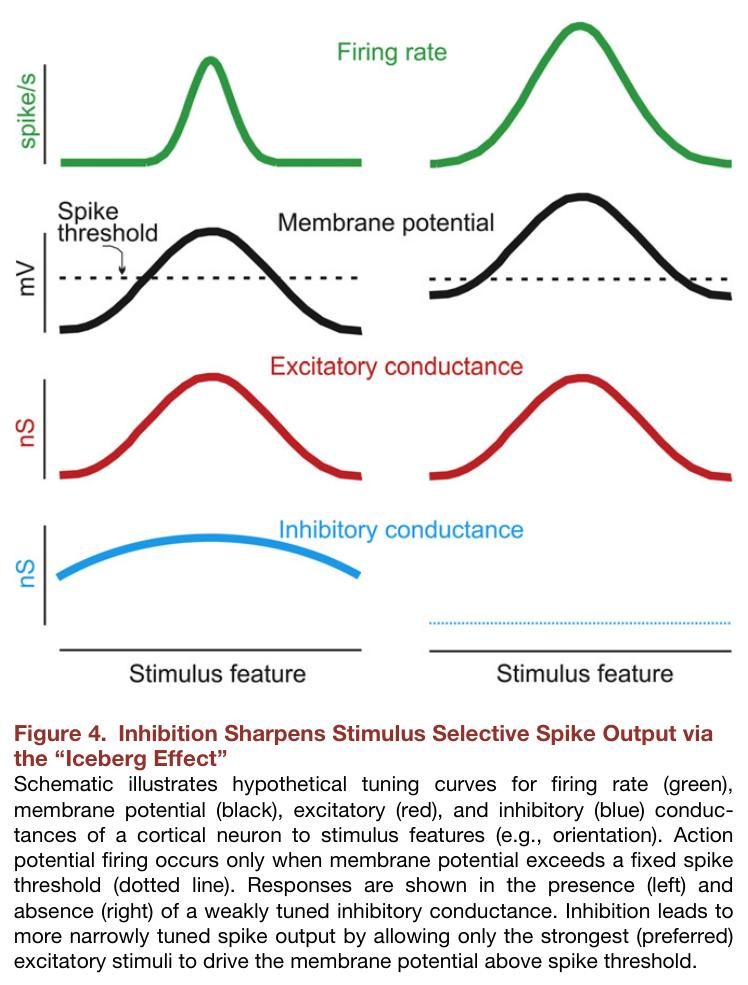
\includegraphics[width=0.6\textwidth, 
		height=0.4\textheight]{../figures/isaacson2001_figure4.jpg}
		\caption{how input sharpens tuning. From \cite{Isaacson2011}}
		\label{fig:feedf}
	\end{figure}
	\begin{itemize}
		\item 
	\end{itemize}
	\subsection{Cross-inhibition}
	\begin{itemize}
		\item 
	\end{itemize}
	\subsection{Feedback inhibition}
	\begin{itemize}
		\item 
	\end{itemize}
	\chapter{Two Mauthner Cells Model}
	\chapter{Coupling of Neuronal Model and Collective Dynamics}
	\chapter{Discussion}
	\begin{itemize}
		\item we focus here on the experimental results from 
		\cite{Bhattacharyya2017} but one should keep in mind that their results 
		might be specific to properties of experiment such as fish handling, 
		fish age, species, arena, environment, stimulus setup (projection on 
		screen)
		\item we took the fitted parameters from \cite{Koyama2016} but those are fitted for their 
		specific context which might vary in other experimental conditions and certainly in other 
		species
		\item furthermore the LIF model makes strong assumptions about the processing power of the 
		neuron which are likely not true. see for example \cite{Koch2000}, and specifically for the 
		M-cell \cite{Medan2017}
	\end{itemize}
	\newpage
	\bibliographystyle{abbrvnat}
	\bibliography{masterthesisbib}
	
	\newpage
	\appendix
	%\appendixheaderon
		% next line tells latex to not list sections in the Table of Contents, \protect is needed because \setcounter apparantly
		% is a fragile command (see http://www.tex.ac.uk/FAQ-protect.html)
	\addtocontents{toc}{\protect\setcounter{tocdepth}{-1}}
	\section{Appendix}

	
\end{document}          
